\documentclass[]{article}
\usepackage[T1]{fontenc}
\usepackage{lmodern}
\usepackage{amssymb,amsmath}
\usepackage{ifxetex,ifluatex}
\usepackage{fixltx2e} % provides \textsubscript
% Set line spacing
% use upquote if available, for straight quotes in verbatim environments
\IfFileExists{upquote.sty}{\usepackage{upquote}}{}
\ifnum 0\ifxetex 1\fi\ifluatex 1\fi=0 % if pdftex
  \usepackage[utf8]{inputenc}
\else % if luatex or xelatex
  \ifxetex
    \usepackage{mathspec}
    \usepackage{xltxtra,xunicode}
  \else
    \usepackage{fontspec}
  \fi
  \defaultfontfeatures{Mapping=tex-text,Scale=MatchLowercase}
  \newcommand{\euro}{€}
\fi
% use microtype if available
\IfFileExists{microtype.sty}{\usepackage{microtype}}{}
\usepackage[margin=1in]{geometry}
\usepackage{color}
\usepackage{fancyvrb}
\newcommand{\VerbBar}{|}
\newcommand{\VERB}{\Verb[commandchars=\\\{\}]}
\DefineVerbatimEnvironment{Highlighting}{Verbatim}{commandchars=\\\{\}}
% Add ',fontsize=\small' for more characters per line
\usepackage{framed}
\definecolor{shadecolor}{RGB}{48,48,48}
\newenvironment{Shaded}{\begin{snugshade}}{\end{snugshade}}
\newcommand{\KeywordTok}[1]{\textcolor[rgb]{0.94,0.87,0.69}{{#1}}}
\newcommand{\DataTypeTok}[1]{\textcolor[rgb]{0.87,0.87,0.75}{{#1}}}
\newcommand{\DecValTok}[1]{\textcolor[rgb]{0.86,0.86,0.80}{{#1}}}
\newcommand{\BaseNTok}[1]{\textcolor[rgb]{0.86,0.64,0.64}{{#1}}}
\newcommand{\FloatTok}[1]{\textcolor[rgb]{0.75,0.75,0.82}{{#1}}}
\newcommand{\CharTok}[1]{\textcolor[rgb]{0.86,0.64,0.64}{{#1}}}
\newcommand{\StringTok}[1]{\textcolor[rgb]{0.80,0.58,0.58}{{#1}}}
\newcommand{\CommentTok}[1]{\textcolor[rgb]{0.50,0.62,0.50}{{#1}}}
\newcommand{\OtherTok}[1]{\textcolor[rgb]{0.94,0.94,0.56}{{#1}}}
\newcommand{\AlertTok}[1]{\textcolor[rgb]{1.00,0.81,0.69}{{#1}}}
\newcommand{\FunctionTok}[1]{\textcolor[rgb]{0.94,0.94,0.56}{{#1}}}
\newcommand{\RegionMarkerTok}[1]{\textcolor[rgb]{0.80,0.80,0.80}{{#1}}}
\newcommand{\ErrorTok}[1]{\textcolor[rgb]{0.76,0.75,0.62}{{#1}}}
\newcommand{\NormalTok}[1]{\textcolor[rgb]{0.80,0.80,0.80}{{#1}}}
\usepackage{graphicx}
% Redefine \includegraphics so that, unless explicit options are
% given, the image width will not exceed the width of the page.
% Images get their normal width if they fit onto the page, but
% are scaled down if they would overflow the margins.
\makeatletter
\def\ScaleIfNeeded{%
  \ifdim\Gin@nat@width>\linewidth
    \linewidth
  \else
    \Gin@nat@width
  \fi
}
\makeatother
\let\Oldincludegraphics\includegraphics
{%
 \catcode`\@=11\relax%
 \gdef\includegraphics{\@ifnextchar[{\Oldincludegraphics}{\Oldincludegraphics[width=\ScaleIfNeeded]}}%
}%
\ifxetex
  \usepackage[setpagesize=false, % page size defined by xetex
              unicode=false, % unicode breaks when used with xetex
              xetex]{hyperref}
\else
  \usepackage[unicode=true]{hyperref}
\fi
\hypersetup{breaklinks=true,
            bookmarks=true,
            pdfauthor={bdanalytics},
            pdftitle={Dutch Environmental Permit Application Process: CoSeLoG},
            colorlinks=true,
            citecolor=blue,
            urlcolor=blue,
            linkcolor=magenta,
            pdfborder={0 0 0}}
\urlstyle{same}  % don't use monospace font for urls
\setlength{\parindent}{0pt}
\setlength{\parskip}{6pt plus 2pt minus 1pt}
\setlength{\emergencystretch}{3em}  % prevent overfull lines
\setcounter{secnumdepth}{5}

%%% Change title format to be more compact
\usepackage{titling}
\setlength{\droptitle}{-2em}
  \title{Dutch Environmental Permit Application Process: CoSeLoG}
  \pretitle{\vspace{\droptitle}\centering\huge}
  \posttitle{\par}
  \author{bdanalytics}
  \preauthor{\centering\large\emph}
  \postauthor{\par}
  \date{}
  \predate{}\postdate{}




\begin{document}

\maketitle


{
\hypersetup{linkcolor=black}
\setcounter{tocdepth}{2}
\tableofcontents
}
\begin{center}\rule{0.5\linewidth}{\linethickness}\end{center}

\textbf{Date: (Thu) Dec 25, 2014}

\section{Background:}\label{background}

Data: Originates from the CoSeLoG project executed under NWO project
number 638.001.211. Within the CoSeLoG project the (dis)similarities
between several processes of different municipalities in the Netherlands
has been investigated. This event log contains the records of the
execution of the receiving phase of the building permit application
process in an anonymous municipality.

Source:
\url{http://data.3tu.nl/repository/uuid:a07386a5-7be3-4367-9535-70bc9e77dbe6}

Time period: 2010-10-02 to 2012-01-23

\section{Synopsis:}\label{synopsis}

Based on analysis utilizing process mining techniques, the CoSeLoG
process may be enhanced with the following recommendations:

\begin{enumerate}
\def\labelenumi{\arabic{enumi}.}
\item
  Normative Model Enhancements:

  1.1 Rename transitions / tasks / activities to highlight nature of
  activity rather than working on a ``receipt'' e.g.~T00 (``Confirmation
  of receipt'') \& T01 through T05.

  1.2 Review need for many ``silent'' transitions \& places. For e.g.
  ``0 sink'', first ``tau split'' and the immediately succeeding places
  called ``source'' might not be really adding much value, especially if
  it's required more for process analytics rather than the actual
  business needs / process.

  1.3. Add guards to decision points utilizing case attributes which
  were either not available / utilized for this analysis.

  1.3. Analyze positive \& negative deviations in real-world cases
  utilizing decision points' guards. Negative deviations should create
  ``alerts'' to the appropriate personnel in real-time. Positive
  deviations should be utilized to enhance the normative model.
\item
  Bottleneck improvements:

  2.1 There are 791 cases that take 79.6 months to traverse from T05 to
  T06 which is approx. 31\% of the duration of all cases. However, this
  path is not allowed by the normative process model. Reducing this
  duration will have a big impact on the overall process duration.

  2.2 Similarly, there are 1,079 cases that take 29.6 months from T00 to
  T02 which is also not allowed by the normative process model.

  2.3 To enhance the process and facilitate further analytics, capture
  transitional information about each task / acitivity (e.g.~start,
  complete, abort, schedule, assign, suspend, resume, withdraw, etc.)
\item
  Resource alloaction / utilization:

  3.1 Categorize resources into ``Generalists'' vs. ``Specialists'' to
  enhance both efficiency and effectiveness.

  3.2 Implement a Resource Recommendation System that considers resource
  type \& capacity along with case attributes \& time deadlines to
  recommend resources for the next event / activity for the case. Broad
  design guidelines may include:

  3.2.A Assign cases that require specialists based on case attributes /
  guards as they evolve in real-time. Once the case is assigned to a
  specialist, increase accountability by ensuring that case is processed
  all the way to completion by that specialist only, as much as
  possible.

  3.2.B If the case does not require a specialist, increase
  accountability by ensuring that case is processed all the way to
  completion by that generalist only, as much as possible.

  3.2.C Reducing the number of hand-offs (as long as that resource has
  capacity) will have a higher probability of identifying inherent
  bottlenecks and other efficiency improvements (e.g.~whenever a new
  resource has to step in for a case, that case needs to be ``learnt''
  by that resource prior to executing any task).
\end{enumerate}

\subsection{Potential next steps
include:}\label{potential-next-steps-include}

\begin{enumerate}
\def\labelenumi{\arabic{enumi}.}
\item
  Utilize ``training'' vs. ``test'' or cross-validation technique(s) to
  discover different Petri nets and collect the generalization
  conformance fitness metric.
\item
  Compute additional Petri net evaluation metrics e.g.
  ``Simplicity.Entropy''
\item
  Discover Petri net in ProM: 1.1 Add
  Fitness/Simplicity/Precision/Generalization to Petri net selection
  criteria.\\1.2 Add place names to discovered Petri nets. 1.3 Radar
  plot of model evaluations. 1.4 Display remaining tokens in selected
  Petri net.
\end{enumerate}

X.1 Review questions in Peer Assignment to ensure that all have been
answered\\X.2 Re-do listed steps to ensure reproduceability\\X.3 Convert
text to tables where appropriate\\X.4 Clean formats to make it more
readable X.5 Scan Peer Assignment Forum for enhancement ideas

\section{Import event log in Disco}\label{import-event-log-in-disco}

\textbf{Approach I used}:\\1. Import the event log into Disco.\\2.
Switch to ``Statistics'' tab / view\\3. Click on ``Overview'' button in
the left pane under ``Statistics views''\\4. Click on ``Events per
case'' button to the left of the graph

\textbf{What I saw}:

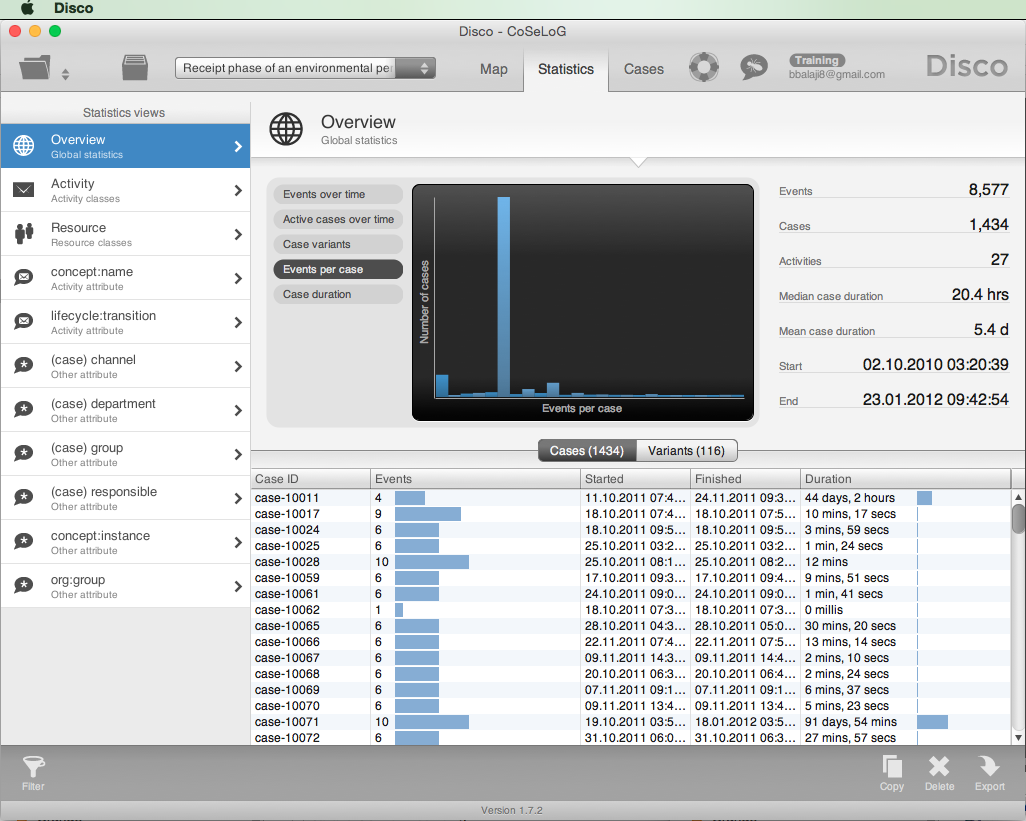
\includegraphics{CoSeLoG_Step_01_Q_01.png}

The graph pane displays a histogram (Number of cases) of Events per case
in this event log. The event log contains 8,577 events in 1,434 cases
with 27 activities.

\textbf{My analysis}:\\There are 6 events on average per case. This
information can be gathered by hovering the mouse on the tallest bar.

By clicking on ``Variants'' button on top of the table, we can see that
there are only 116 variants amongst the 1,434 cases.

The main observation from the `Events over time' graph is that the
maximum number of events (77) occured on Apr 27, 2011 across cases.

\section{Analyze process map in
Disco}\label{analyze-process-map-in-disco}

\textbf{Approach I used}:\\1. Click on ``Map'' tab in the window
header.\\2. Set ``Activities'' slider to 0\% \& ``Paths'' slider to 50\%
to make the process map fit on one screen and still be readable.

\textbf{What I saw}:

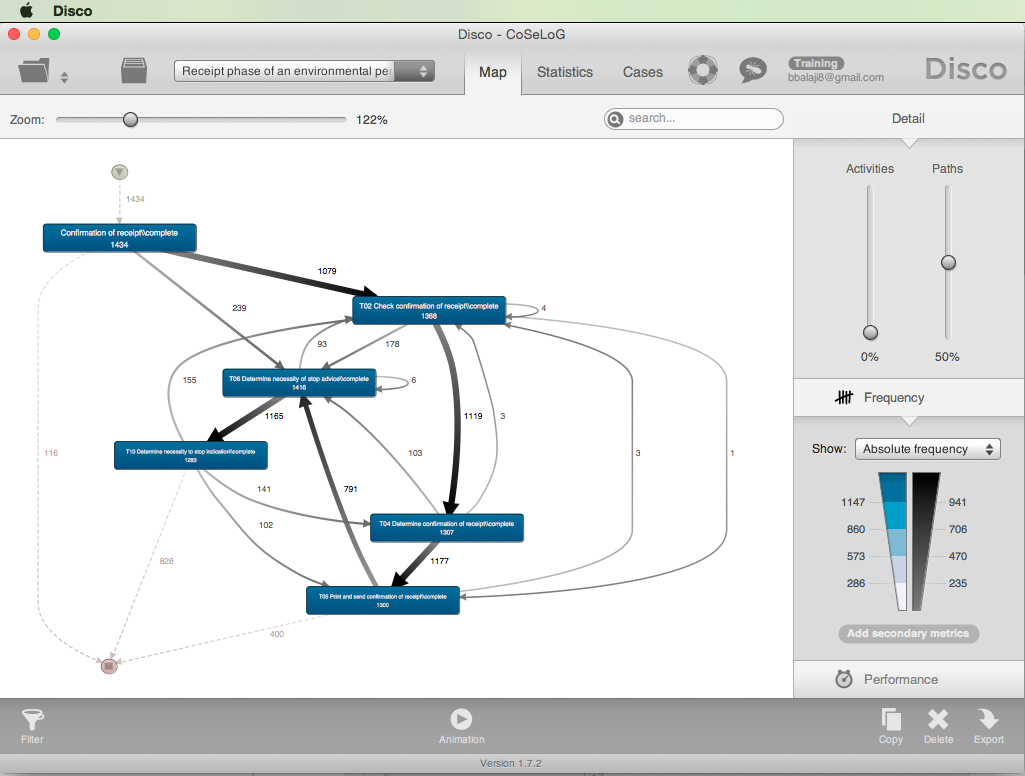
\includegraphics{CoSeLoG_Step_02.png}

\textbf{My analysis}:

The 6 most frequent activities between the initiation and termination of
cases in the process map include:\\A. Confirmation of receipt (labeled
as ``T00'' in the rest of this document)\\B. T02 Check confirmation of
receipt\\C. T04 Determine confirmation of receipt\\D. T05 Print and send
confirmation of receipt\\E. T06 Determine necessity of stop advice\\F.
T10 Determine necessity to stop indication

The most frequent activity paths traced by the cases include:

\begin{verbatim}
##                                           Activity.Path Cases
##                                     Start -> T00 -> End   116
##                Start -> T00 -> T02 -> T04 -> T05 -> End   400
##  Start -> T00 -> T02 -> T04 -> T05 -> T06 -> T10 -> End   828
\end{verbatim}

These traces capture 93.7 \% of the cases in the event log. There are 4
activities (T00, T02, T04 \& T05) regarding confirmation of receipts.
Maybe these activities are not named appropriately ?

\section{Analyze process performance in
Disco}\label{analyze-process-performance-in-disco}

\textbf{Approach I used}:\\1. Click on ``Performance'' bar / button in
the ``Detail'' pane (right above the ``Copy'' / ``Delete'' / ``Export''
icons).\\2. Select ``Total Duration'' in the ``Performance'' pane to
display.\\3. Select ``Case frequency'' as the secondary metric in the
``Performance'' pane to ensure that we don't use outliers (e.g.~low case
frequency) to make broad conclusions about the process.\\4. Cycle
through different metrics in the button next to ``Show:'' in the
Performance pane.

\textbf{What I saw}:

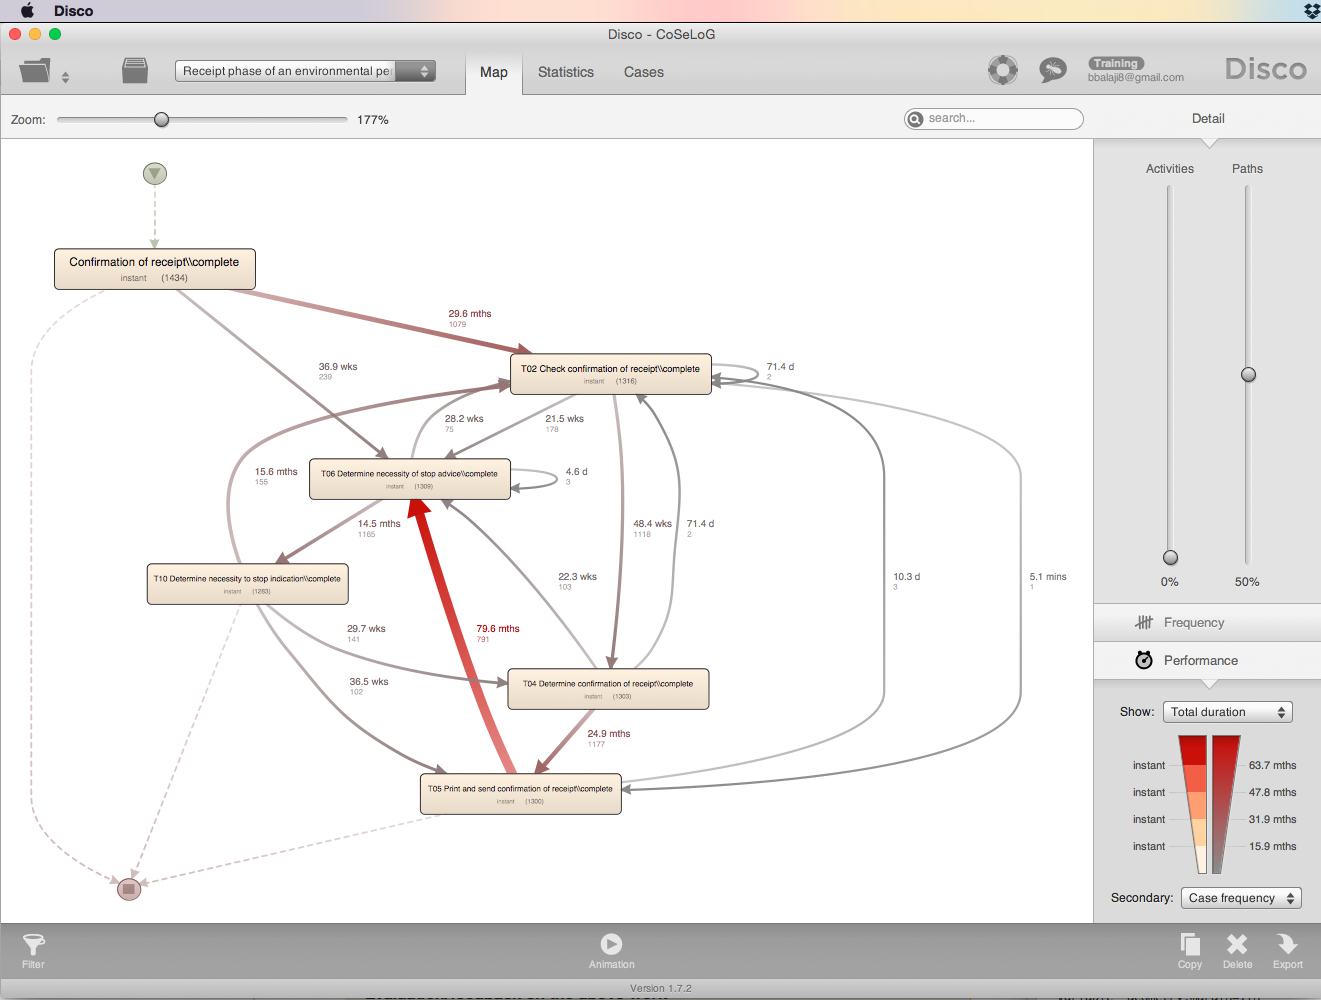
\includegraphics{CoSeLoG_Step_03.png}

The color \& thickness of the arcs are based on the distribution of the
selected primary performance metric. Additionally, if an arc is clicked,
a statistics window is displayed for that arc.

\textbf{My analysis}:\\\emph{Total Duration}: The arc from T05 to T06
takes 79.6 months for 791 cases (31\% of total duration of all cases
which is 258.12 months: mean of 5.4 days per case X 1,434 cases / 30
elapsed days per month). The next bottleneck seems to be T00
-\textgreater{} T02 which is 29.6 months for 1,079 cases.

Analysis of other metrics (median, mean \& max duration) highlighted
arcs with very low case frequency.

\section{Analyze event log in ProM}\label{analyze-event-log-in-prom}

\textbf{Approach I used}:

\begin{enumerate}
\def\labelenumi{\arabic{enumi}.}
\itemsep1pt\parskip0pt\parsep0pt
\item
  Click on ``import\ldots{}'' icon on the upper right hand side of the
  ``Workspace'' pane.\\
\item
  Click on eye icon (the one associated with the log in the middle; NOT
  the top one).
\item
  Click on ``Create new\ldots{}'' droplist in the top center of the
  window.
\item
  Select ``XDotted Chart'' by scrolling down the list.
\item
  Select ``Dotted Chart'' tab on the left.
\item
  Select ``Occurence of first event'' from the droplist for ``Case
  order:'' option.
\item
  Click on ``Apply Settings'' button.
\end{enumerate}

\textbf{What I saw}:

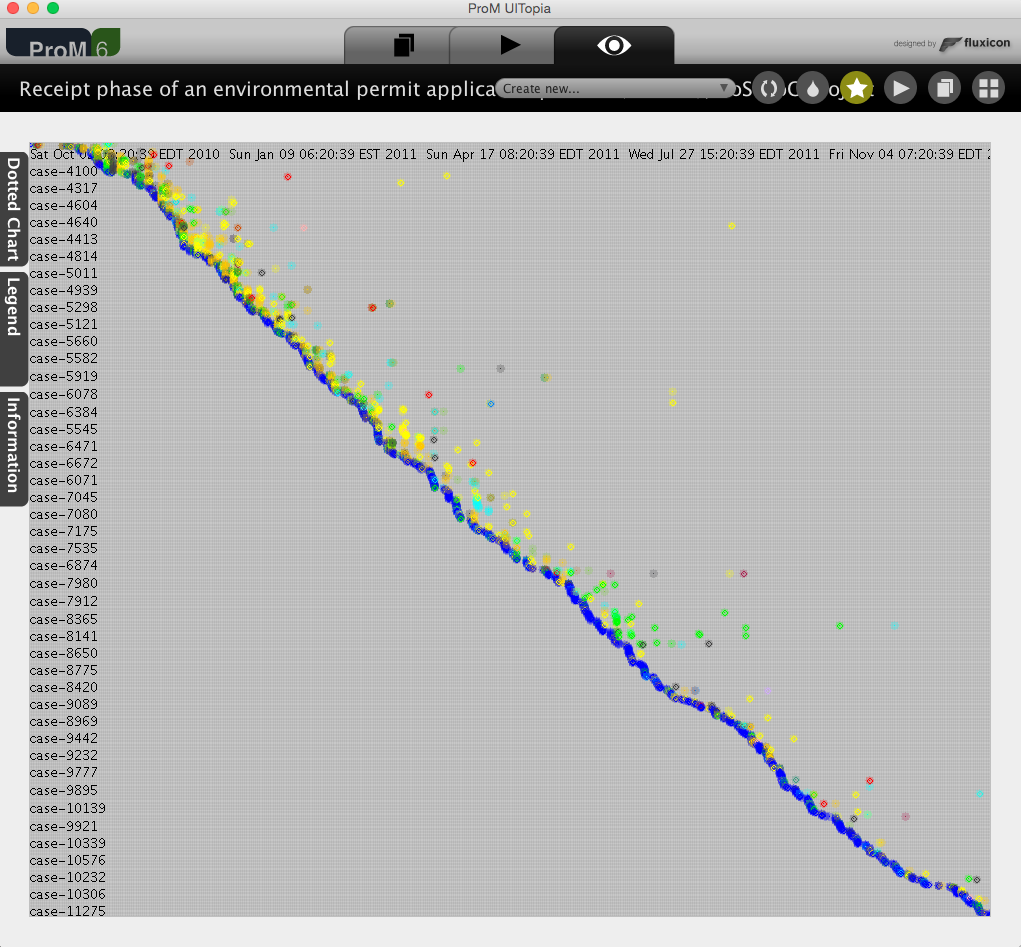
\includegraphics{CoSeLoG_Step_04.png}

Events for each case are plotted across time and color-coded. Zooming in
does not make the timeline any more readable / discernible (e.g.~do
events initiate on weekends ?)

\textbf{My analysis}:\\The arrival of the new cases is fairly constant
evidenced by the -45 degree slope of the (approx) line of blue dots.
There are some minor fluctuations which is difficult to quantify
(clicking on the dots does not display any additional information).

For the more recent cases there are a lot less events / activities
occuring close to case initiation compared to the earlier cases.

\section{Discover Petri net in ProM}\label{discover-petri-net-in-prom}

\subsection{Alpha Algorithm}\label{alpha-algorithm}

\textbf{Approach I used}:

\begin{enumerate}
\def\labelenumi{\arabic{enumi}.}
\itemsep1pt\parskip0pt\parsep0pt
\item
  Click on ``Actions'' icon.
\item
  Add imported event log to ``Input''.
\item
  Search for ``Alpha'' plug-in.
\item
  Select ``Mine for a Petri Net using Alpha-algorithm''.
\item
  Click on ``Start'' button.
\end{enumerate}

\textbf{What I saw}:

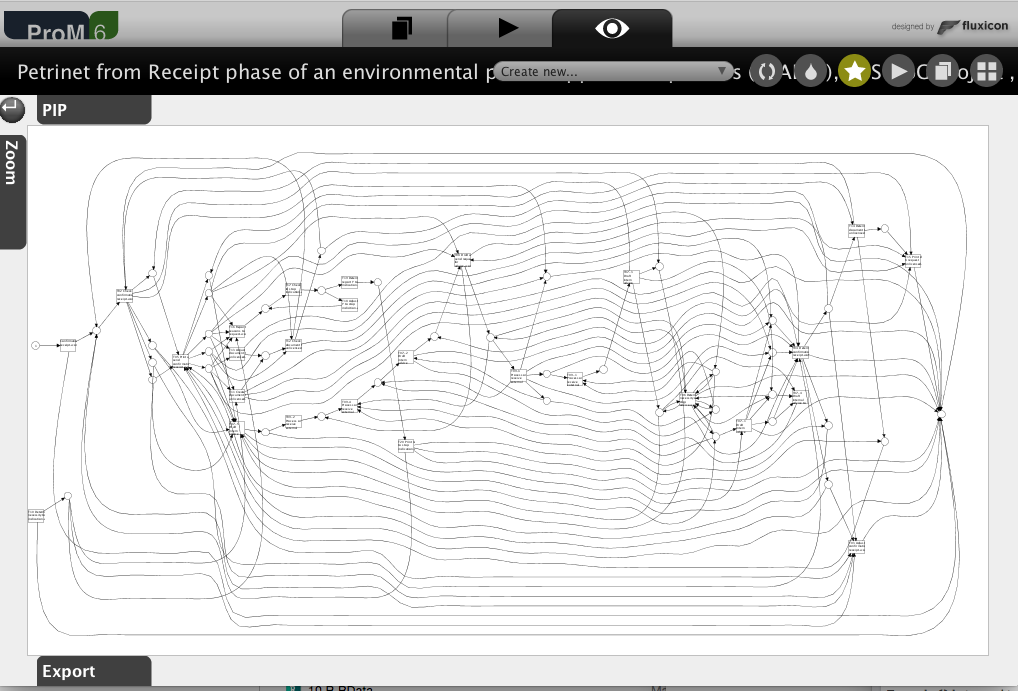
\includegraphics{CoSeLoG_Step_05.png}

This is clearly difficult to work with. Let's filter the event log to
make it more comprehensible.

\textbf{Approach I used}:

\begin{enumerate}
\def\labelenumi{\arabic{enumi}.}
\setcounter{enumi}{9}
\itemsep1pt\parskip0pt\parsep0pt
\item
  Click on ``Actions'' icon.
\item
  Search for ``Filter Log''.
\item
  Select ``Filter Log using Simple Heuristics''.
\item
  Click on ``Start'' button.
\item
  Change Log name to ``CoSeLoG (filtered on simple heuristics)''.
\item
  Click on ``Next'' button.
\item
  Select ``Select top percentage'' to 100\% because there is only 1
  Start event.
\item
  Click on ``Next'' button.
\item
  Select ``Select top percentage'' to 100\% because ideally keeping all
  End events would be critical in understanding the process.
\item
  Click on ``Next'' button.
\item
  Select ``Select top percentage'' to 96\% because this Event filter
  criterion discards many events and therefore many arcs in the
  resulting Petri net. 97\% filtering results in a much more complex
  Petri net.\\
\item
  Change Log name to ``CoSeLoG (96\% filtered on simple heuristics)''.
\item
  Click on ``Finish'' button.
\end{enumerate}

\textbf{What I saw}:

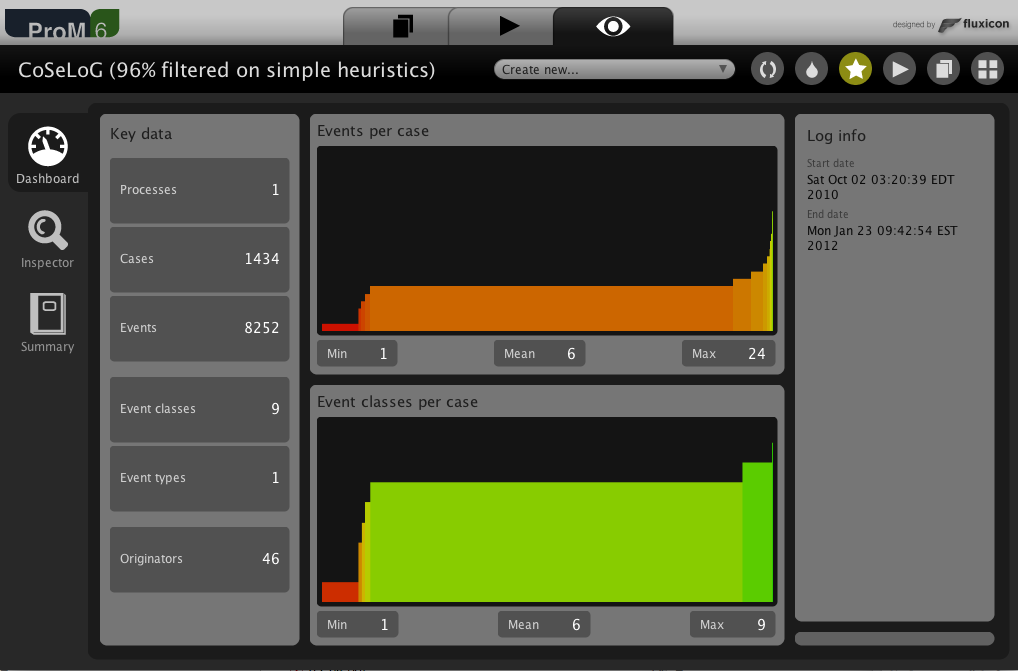
\includegraphics{CoSeLoG_Step_05_Filter96.png}

The number of Event classes has gone down from 27 to 9. The number of
Events has reduced from 8,577 to 8,252 but number of Cases remain the
same. Now, let's see if we can discover a simpler Petri net.

\textbf{Approach I used}:

Repeat actions numbered 1-5 listed earlier in this section utilizing the
``CoSeLoG (96\% filtered\ldots{})'' log.

\textbf{What I saw}:

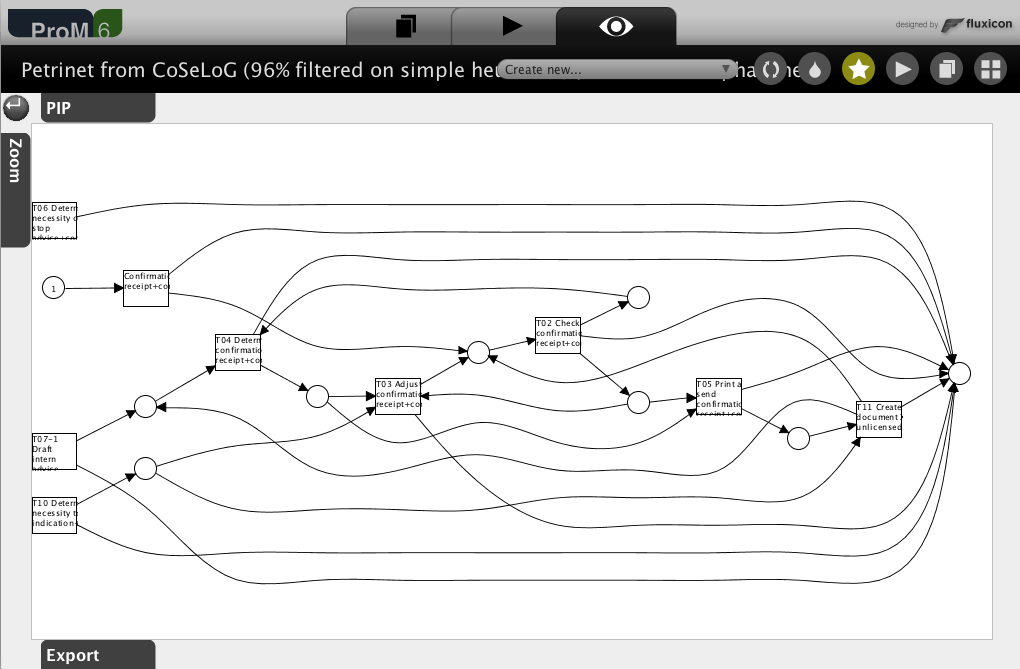
\includegraphics{CoSeLoG_Step_05_Filter96_PetriNet_Alpha.png}

The Alpha algorithm has discovered 9 transitions \& 9 places. However,
transitions T06, T07-1 \& T10 are not integrated well into the rest of
the control-flow. Collect Petri net evaluation metrics as listed in the
Appendix section ``Actions to run ProM plug-in''Replay a Log on Petri
Net for Conformance Analysis``''.

\textbf{My analysis}:

\begin{verbatim}
##  Petrinet Fitness.Traces Simplicity.Places.Total
##     Alpha         0.8987                       9
##  Simplicity.Places.Implicit Simplicity.Transitions.Silent Simplicity.Arcs
##                           0                             0              30
##  Simplicity.MDL Generalization.Conformance Precision.Behavioral
##               1                     0.8987               0.1971
\end{verbatim}

Strictly speaking, the ``Generalization.Conformance'' metric would
typically be lower than ``Fitness.Traces'' if the proper ``training''
vs. ``test'' events log technique or the cross-validation technique is
utilized for discovering the Petri net and then testing for conformance.
This analysis collects this metric for the sake of analysis completeness
without utilizing those techniques (a lot of work !).

\subsection{ILP}\label{ilp}

\textbf{Approach I used}:

\begin{enumerate}
\def\labelenumi{\arabic{enumi}.}
\itemsep1pt\parskip0pt\parsep0pt
\item
  Click on ``Actions'' icon.
\item
  Add ``CoSeLoG (96\% filtered\ldots{})'' log to ``Input''.\\
\item
  Search for ``ILP'' plug-in.
\item
  Select ``Mine for a Petri Net using ILP''.
\item
  Click on ``Start'' button.
\item
  Select the ``Number of places'' option to ``Before \& After
  Transition'' instead of ``Per Causal Dependency'' to ensure clear
  ``End'' states \& minimize number of arcs.
\item
  Click ``Finish'' button.
\end{enumerate}

\textbf{What I saw}:

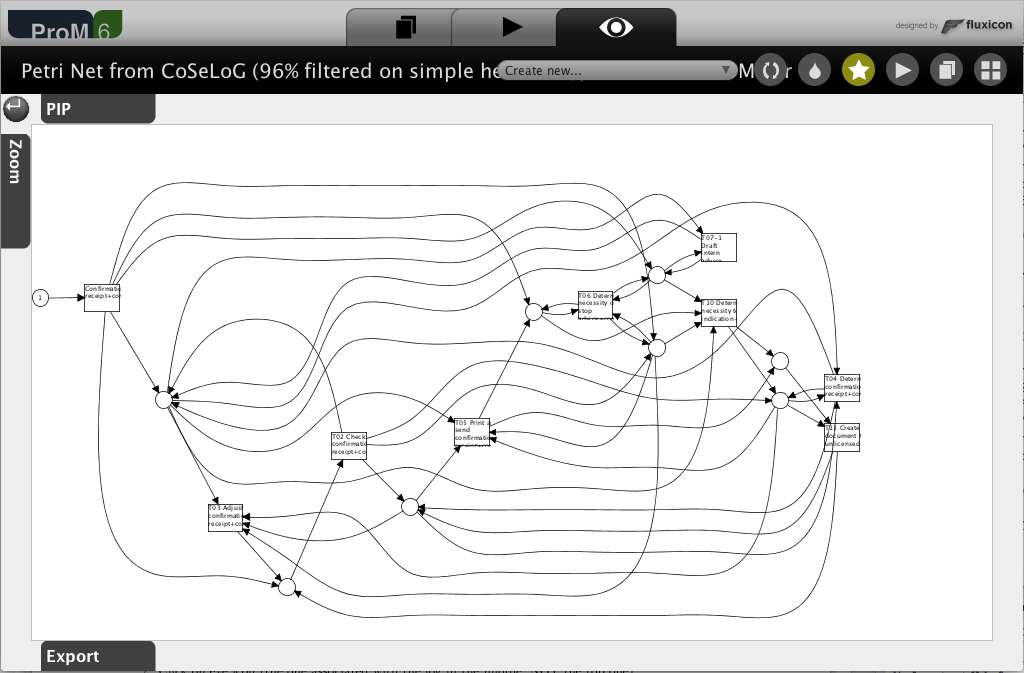
\includegraphics{CoSeLoG_Step_05_Filter96_PetriNet_ILP.png}

The ILP algorithm has discovered 9 transitions \& 8 places (``P 1'' \&
``P 2'' are ``End'' places). Additionally, the ILP Petri net handles
transitions T06, T07-1 \& T10 better by not isolating them from the
control-flow. Collect Petri net evaluation metrics as listed in the
Appendix section ``Actions to run ProM plug-in''Replay a Log on Petri
Net for Conformance Analysis``''.

\textbf{My analysis}:

\begin{verbatim}
##  Petrinet Fitness.Traces Simplicity.Places.Total
##       ILP         0.8483                       8
##  Simplicity.Places.Implicit Simplicity.Transitions.Silent Simplicity.Arcs
##                           0                             0              21
##  Simplicity.MDL Generalization.Conformance Precision.Behavioral
##               3                     0.8483               0.9955
\end{verbatim}

\subsection{Heuristics Miner}\label{heuristics-miner}

\textbf{Approach I used}:

\begin{enumerate}
\def\labelenumi{\arabic{enumi}.}
\itemsep1pt\parskip0pt\parsep0pt
\item
  Click on ``Actions'' icon.
\item
  Add ``CoSeLoG (96\% filtered\ldots{})'' log to ``Input''.
\item
  Search for ``Heuristics'' plug-in.
\item
  Select ``Mine for a Heuristics Net using Heuristics Miner''.
\item
  Click on ``Start'' button.
\item
  Select the default options and Click ``Continue'' button.
\item
  Click on ``Zoom'' button to the left of the graphic.
\item
  Select zoom level next to ``Fit \textgreater{}'' on the slider to view
  the net in its entirety.
\item
  Capture screen image.
\item
  Select zoom level to 50\% to make the net more readable.
\end{enumerate}

\textbf{What I saw}:

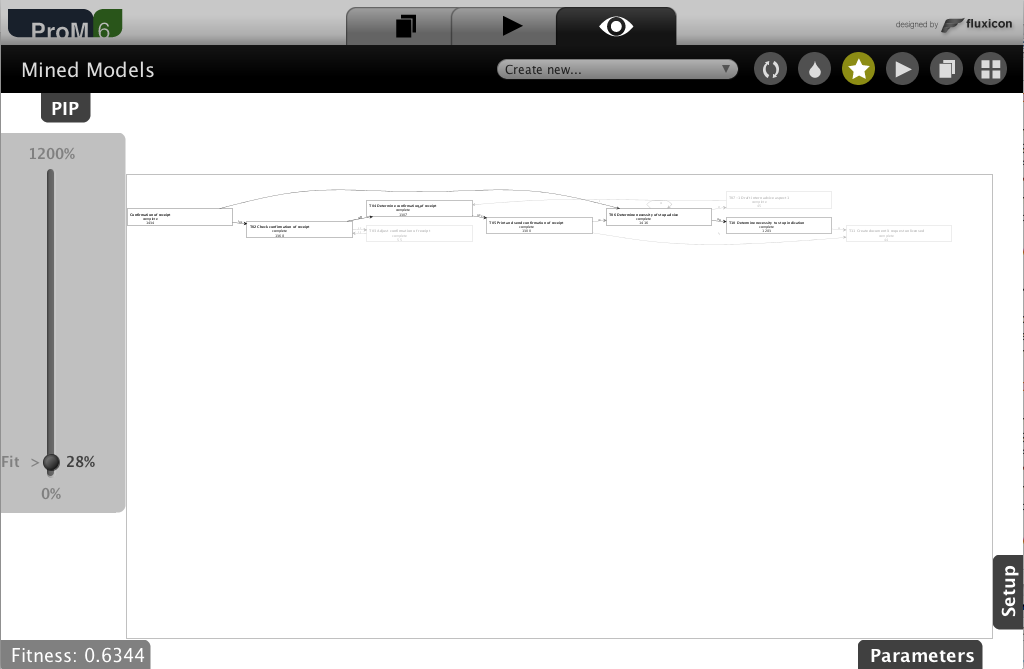
\includegraphics{CoSeLoG_Step_05_Filter96_Heuristics_Net.png}

9 transitions are discovered with a fitness score of 0.63 but T03, T07-1
\& T11 are grayed out due to low case frequency (\textless{}= 55).

\textbf{Approach I used}:

\begin{enumerate}
\def\labelenumi{\arabic{enumi}.}
\setcounter{enumi}{19}
\itemsep1pt\parskip0pt\parsep0pt
\item
  Click on ``Workspace'' icon.
\item
  Select ``Mined Models'' of type ``HeuristicsNet''.
\item
  Click on ``Actions'' icon.
\item
  Select ``Convert Heuristics net into Petri net'' plug-in.
\item
  Click on ``Start'' button.
\end{enumerate}

\textbf{What I saw}:

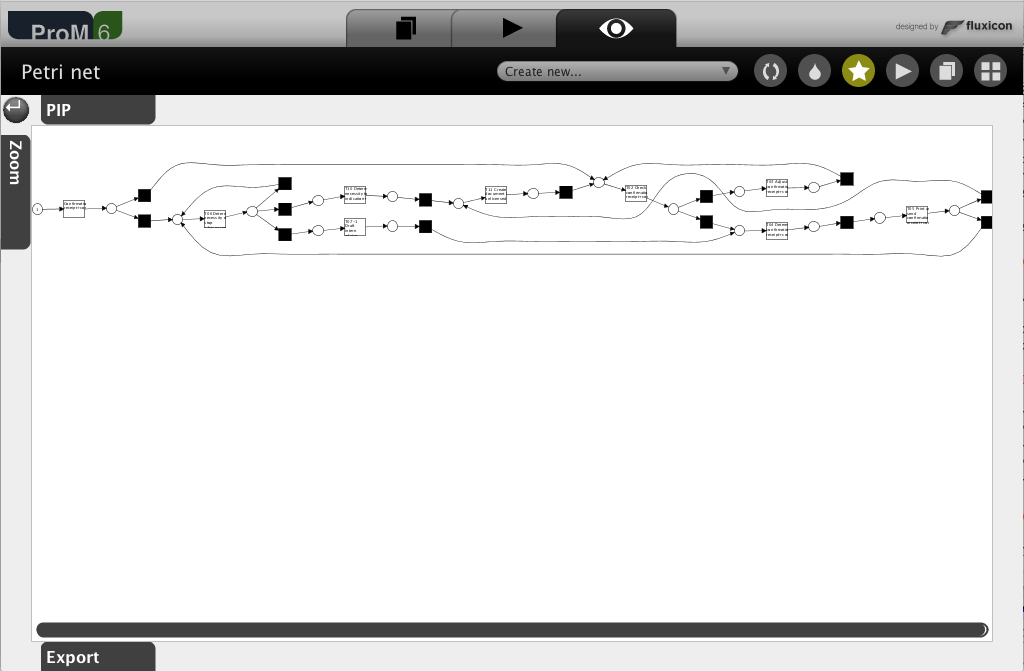
\includegraphics{CoSeLoG_Step_05_Filter96_PetriNet_Heuristics.png}

This approach has discovered 9 transitions again, 14 ``hidden'' /
``silent'' transitions and 18 places. However, there does not seem to be
a clear ``End'' place. It appears that ``pi1'' is the closest ``End''
place.

\textbf{My analysis}:

\begin{verbatim}
##    Petrinet Fitness.Traces Simplicity.Places.Total
##  Heuristics         0.7698                      18
##  Simplicity.Places.Implicit Simplicity.Transitions.Silent Simplicity.Arcs
##                           0                            14              44
##  Simplicity.MDL Generalization.Conformance Precision.Behavioral
##               2                     0.7698               0.8656
\end{verbatim}

\subsection{Inductive Miner}\label{inductive-miner}

\textbf{Approach I used}:

\begin{enumerate}
\def\labelenumi{\arabic{enumi}.}
\itemsep1pt\parskip0pt\parsep0pt
\item
  Click on ``Workspace'' icon.
\item
  Select ``CoSeLoG (96\% filtered\ldots{})'' log.
\item
  Click on ``Actions'' icon.
\item
  Search for ``Inductive'' plug-in.
\item
  Select ``Mine Petri net with Inductive Miner'' plug-in.
\item
  Click on ``Start'' button.
\item
  Change ``Variant'' option from default of ``Inductive Miner -
  infrequent'' to ``Inductive Miner'' because the default option drops
  T04 transition probably due to infrequent cases containing it. We want
  to keep this transition so that we can compare the different Petri
  nets with the same set of transitions.
\item
  Click ``Finish'' button.
\end{enumerate}

\textbf{What I saw}:

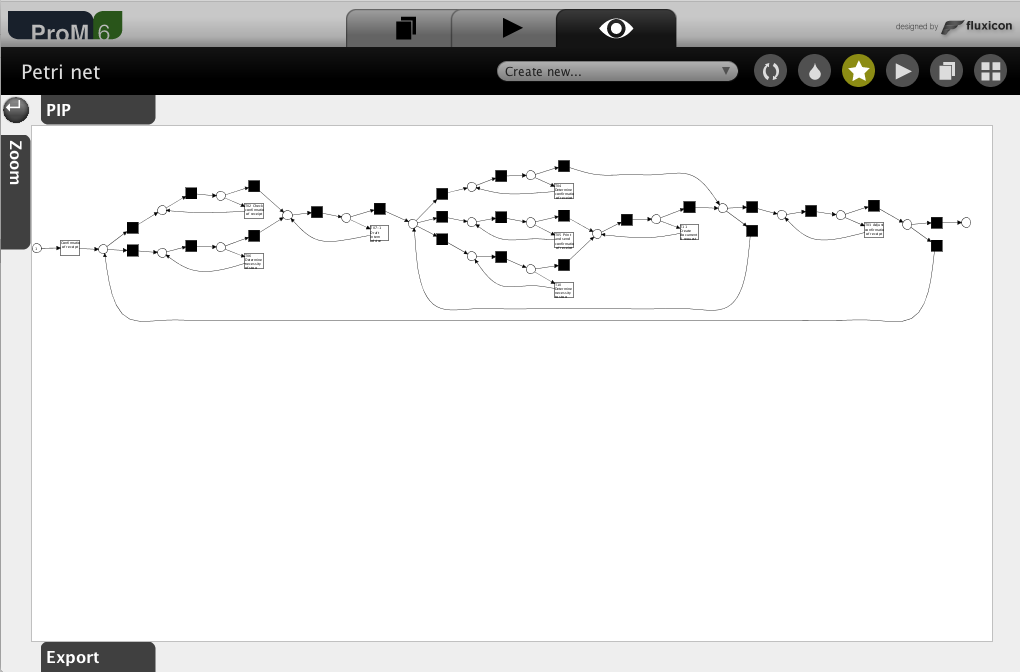
\includegraphics{CoSeLoG_Step_05_Filter96_PetriNet_Inductive.png}

This approach discovered 9 transitions, 25 ``hidden'' / ``silent''
transitions \& 21 places. The ``End'' place is named as ``sink''.

\textbf{My analysis}:

\begin{verbatim}
##   Petrinet Fitness.Traces Simplicity.Places.Total
##  Inductive         0.9813                      21
##  Simplicity.Places.Implicit Simplicity.Transitions.Silent Simplicity.Arcs
##                           0                            25              68
##  Simplicity.MDL Generalization.Conformance Precision.Behavioral
##              13                     0.9813               0.9955
\end{verbatim}

\subsection{Select ``Best'' Petri net}\label{select-best-petri-net}

\textbf{My analysis}:

The metrics for all the discovered Petri nets:

\begin{verbatim}
##            Fitness.Traces Simplicity.Places.Total
## Alpha              0.8987                       9
## ILP                0.8483                       8
## Heuristics         0.7698                      18
## Inductive          0.9813                      21
##            Simplicity.Places.Implicit Simplicity.Transitions.Silent
## Alpha                               0                             0
## ILP                                 0                             0
## Heuristics                          0                            14
## Inductive                           0                            25
##            Simplicity.Arcs Simplicity.MDL Generalization.Conformance
## Alpha                   30              1                     0.8987
## ILP                     21              3                     0.8483
## Heuristics              44              2                     0.7698
## Inductive               68             13                     0.9813
##            Precision.Behavioral
## Alpha                    0.1971
## ILP                      0.9955
## Heuristics               0.8656
## Inductive                0.9955
\end{verbatim}

To consolidate the Simplicity.* metrics into a Simplicity.Score for each
Petri net, assign equal weights (as a simple approximation) by scaling
the raw metric relative to a ``perfect'' score of 100 since each metric
has different scales. For e.g.~the minimum value of
Simplicity.Places.Total is 8 which may be considered as the ``perfect''
score amongst these Petri nets. If the minimum value is 0 we add 1 to
both numerator \& denominator.

\begin{Shaded}
\begin{Highlighting}[]
\NormalTok{consolidate_scores <-}\StringTok{ }\NormalTok{function(pn_df, metrics, consolidated.metric.name) \{}
    
    \NormalTok{for (metric in metrics) \{}
        \NormalTok{min_value <-}\StringTok{ }\KeywordTok{min}\NormalTok{(pn_df[, metric])}
        
        \NormalTok{if(min_value ==}\StringTok{ }\DecValTok{0}\NormalTok{) \{}
            \CommentTok{# Add 1 to account for possibility of 0 in denominator}
            \NormalTok{pn_df[, }\KeywordTok{paste0}\NormalTok{(metric, }\StringTok{".Scaled"}\NormalTok{)] <-}\StringTok{ }
\StringTok{                }\NormalTok{((min_value +}\StringTok{ }\DecValTok{1}\NormalTok{) *}\StringTok{ }\FloatTok{100.0}\NormalTok{) /}\StringTok{ }\NormalTok{(pn_df[, metric] +}\StringTok{ }\DecValTok{1}\NormalTok{)}
        \NormalTok{\} else \{}
            \NormalTok{pn_df[, }\KeywordTok{paste0}\NormalTok{(metric, }\StringTok{".Scaled"}\NormalTok{)] <-}\StringTok{ }
\StringTok{                }\NormalTok{((min_value +}\StringTok{ }\DecValTok{0}\NormalTok{) *}\StringTok{ }\FloatTok{100.0}\NormalTok{) /}\StringTok{ }\NormalTok{(pn_df[, metric] +}\StringTok{ }\DecValTok{0}\NormalTok{)}
        \NormalTok{\}}
            
    \NormalTok{\}}
    
    \NormalTok{for (row in }\DecValTok{1}\NormalTok{:}\KeywordTok{nrow}\NormalTok{(pn_df))}
        \NormalTok{pn_df[row, consolidated.metric.name] <-}\StringTok{ }
\StringTok{            }\KeywordTok{mean}\NormalTok{(}\KeywordTok{as.numeric}\NormalTok{(pn_df[row, }\KeywordTok{paste0}\NormalTok{(metrics, }\StringTok{".Scaled"}\NormalTok{)]))}

    \NormalTok{ycol_names <-}\StringTok{ }\KeywordTok{c}\NormalTok{(}\StringTok{"Simplicity.Places.Total"}\NormalTok{, }\StringTok{"Simplicity.Places.Total.Scaled"}\NormalTok{,}
                    \StringTok{"Simplicity.Places.Implicit"}\NormalTok{, }\StringTok{"Simplicity.Places.Implicit.Scaled"}\NormalTok{,}
                    \StringTok{"Simplicity.Transitions.Silent"}\NormalTok{, }\StringTok{"Simplicity.Transitions.Silent.Scaled"}\NormalTok{,}
                    \StringTok{"Simplicity.Arcs"}\NormalTok{, }\StringTok{"Simplicity.Arcs.Scaled"}\NormalTok{,}
                    \StringTok{"Simplicity.MDL"}\NormalTok{, }\StringTok{"Simplicity.MDL.Scaled"}
                    \NormalTok{)    }
    \NormalTok{hbar_df <-}\StringTok{ }\KeywordTok{melt}\NormalTok{(}\KeywordTok{cbind}\NormalTok{(}\KeywordTok{data.frame}\NormalTok{(}\DataTypeTok{Petrinet=}\KeywordTok{rownames}\NormalTok{(pn_df)),}
                          \NormalTok{pn_df), }\DataTypeTok{id=}\StringTok{"Petrinet"}\NormalTok{, }\DataTypeTok{measure=}\NormalTok{ycol_names)}
    \NormalTok{hbar_df$variable <-}\StringTok{ }\KeywordTok{as.character}\NormalTok{(hbar_df$variable)}
    \NormalTok{hbar_df$var_type <-}\StringTok{ }\KeywordTok{sapply}\NormalTok{(}\DecValTok{1}\NormalTok{:}\KeywordTok{nrow}\NormalTok{(hbar_df), function(row)}
            \KeywordTok{ifelse}\NormalTok{(}\KeywordTok{length}\NormalTok{(}\KeywordTok{grep}\NormalTok{(}\StringTok{".Scaled"}\NormalTok{, hbar_df[row, }\StringTok{"variable"}\NormalTok{], }\DataTypeTok{fixed=}\OtherTok{TRUE}\NormalTok{)) ==}\StringTok{ }\DecValTok{0}\NormalTok{,}
                            \StringTok{"Simplicity.Raw"}\NormalTok{, }\StringTok{"Simplicity.Scaled"}\NormalTok{))}
    \NormalTok{hbar_df$var_label <-}\StringTok{ }
\StringTok{        }\KeywordTok{gsub}\NormalTok{(}\StringTok{"Simplicity."}\NormalTok{, }\StringTok{""}\NormalTok{,}
            \KeywordTok{sapply}\NormalTok{(}\DecValTok{1}\NormalTok{:}\KeywordTok{nrow}\NormalTok{(hbar_df), function(row)}
            \KeywordTok{ifelse}\NormalTok{(}\KeywordTok{length}\NormalTok{(}\KeywordTok{grep}\NormalTok{(}\StringTok{".Scaled"}\NormalTok{, hbar_df[row, }\StringTok{"variable"}\NormalTok{], }\DataTypeTok{fixed=}\OtherTok{TRUE}\NormalTok{)) ==}\StringTok{ }\DecValTok{0}\NormalTok{,}
                            \NormalTok{hbar_df[row, }\StringTok{"variable"}\NormalTok{], }
                            \KeywordTok{gsub}\NormalTok{(}\StringTok{".Scaled"}\NormalTok{, }\StringTok{""}\NormalTok{, hbar_df[row, }\StringTok{"variable"}\NormalTok{], }\DataTypeTok{fixed=}\OtherTok{TRUE}\NormalTok{))}
                    \NormalTok{),}
            \DataTypeTok{fixed=}\OtherTok{TRUE}\NormalTok{)}
    \NormalTok{gp <-}\StringTok{ }\KeywordTok{ggplot}\NormalTok{(hbar_df, }\KeywordTok{aes}\NormalTok{(}\DataTypeTok{x=}\KeywordTok{reorder}\NormalTok{(Petrinet, value), }\DataTypeTok{y=}\NormalTok{value)) +}\StringTok{       }
\StringTok{            }\KeywordTok{geom_bar}\NormalTok{(}\DataTypeTok{stat=}\StringTok{"identity"}\NormalTok{, }\KeywordTok{aes}\NormalTok{(}\DataTypeTok{fill=}\NormalTok{var_label)) +}\StringTok{ }\KeywordTok{xlab}\NormalTok{(}\StringTok{"Petrinet"}\NormalTok{) +}\StringTok{ }
\StringTok{            }\KeywordTok{facet_grid}\NormalTok{(var_label ~}\StringTok{ }\NormalTok{var_type, }\DataTypeTok{scales=}\StringTok{"free"}\NormalTok{) +}\StringTok{ }
\StringTok{            }\KeywordTok{theme}\NormalTok{(}\DataTypeTok{legend.position=}\StringTok{"none"}\NormalTok{) +}\StringTok{ }\KeywordTok{coord_flip}\NormalTok{()}
    \KeywordTok{print}\NormalTok{(gp)}

    \NormalTok{radar_inp_df <-}\StringTok{ }\KeywordTok{cbind}\NormalTok{( }\KeywordTok{data.frame}\NormalTok{(}\DataTypeTok{instance=}\KeywordTok{rownames}\NormalTok{(pn_df)),}
                                    \KeywordTok{subset}\NormalTok{(pn_df, }\DataTypeTok{select=}\KeywordTok{c}\NormalTok{( }
                                        \NormalTok{Simplicity.Places.Total.Scaled,}
                                        \NormalTok{Simplicity.Places.Implicit.Scaled,}
                                        \NormalTok{Simplicity.Transitions.Silent.Scaled,}
                                        \NormalTok{Simplicity.Arcs.Scaled,}
                                        \NormalTok{Simplicity.MDL.Scaled)),}
                                    \KeywordTok{data.frame}\NormalTok{(}\DataTypeTok{facet=}\KeywordTok{rep}\NormalTok{(}\StringTok{" "}\NormalTok{, }\KeywordTok{nrow}\NormalTok{(pn_df))))}
    \KeywordTok{print}\NormalTok{(}\KeywordTok{myplot_radar}\NormalTok{(radar_inp_df))}

    \KeywordTok{print}\NormalTok{(}\KeywordTok{myplot_hbar}\NormalTok{(pn_df, }\StringTok{".rownames"}\NormalTok{, }\StringTok{"Simplicity.Score"}\NormalTok{))}
    
    \KeywordTok{return}\NormalTok{(pn_df)}
\NormalTok{\}}
\NormalTok{petrinets_mod_df <-}\StringTok{ }\KeywordTok{consolidate_scores}\NormalTok{(}\DataTypeTok{pn_df=}\NormalTok{petrinets_df, }
        \DataTypeTok{metrics=}\KeywordTok{grep}\NormalTok{(}\StringTok{"Simplicity."}\NormalTok{, }\KeywordTok{names}\NormalTok{(petrinets_df), }\DataTypeTok{fixed=}\OtherTok{TRUE}\NormalTok{, }\DataTypeTok{value=}\OtherTok{TRUE}\NormalTok{), }
        \DataTypeTok{consolidated.metric.name=}\StringTok{"Simplicity.Score"}\NormalTok{)}
\end{Highlighting}
\end{Shaded}

\includegraphics{CoSeLoG_files/figure-latex/Select_Petrinet_2-1.pdf}

\begin{verbatim}
## Warning: Removed 15 rows containing missing values (geom_text).
\end{verbatim}

\includegraphics{CoSeLoG_files/figure-latex/Select_Petrinet_2-2.pdf}
\includegraphics{CoSeLoG_files/figure-latex/Select_Petrinet_2-3.pdf}

\begin{Shaded}
\begin{Highlighting}[]
\KeywordTok{print}\NormalTok{(petrinets_mod_df)}
\end{Highlighting}
\end{Shaded}

\begin{verbatim}
##            Fitness.Traces Simplicity.Places.Total
## Alpha              0.8987                       9
## ILP                0.8483                       8
## Heuristics         0.7698                      18
## Inductive          0.9813                      21
##            Simplicity.Places.Implicit Simplicity.Transitions.Silent
## Alpha                               0                             0
## ILP                                 0                             0
## Heuristics                          0                            14
## Inductive                           0                            25
##            Simplicity.Arcs Simplicity.MDL Generalization.Conformance
## Alpha                   30              1                     0.8987
## ILP                     21              3                     0.8483
## Heuristics              44              2                     0.7698
## Inductive               68             13                     0.9813
##            Precision.Behavioral Simplicity.Places.Total.Scaled
## Alpha                    0.1971                       88.88889
## ILP                      0.9955                      100.00000
## Heuristics               0.8656                       44.44444
## Inductive                0.9955                       38.09524
##            Simplicity.Places.Implicit.Scaled
## Alpha                                    100
## ILP                                      100
## Heuristics                               100
## Inductive                                100
##            Simplicity.Transitions.Silent.Scaled Simplicity.Arcs.Scaled
## Alpha                                100.000000               70.00000
## ILP                                  100.000000              100.00000
## Heuristics                             6.666667               47.72727
## Inductive                              3.846154               30.88235
##            Simplicity.MDL.Scaled Simplicity.Score
## Alpha                 100.000000         91.77778
## ILP                    33.333333         86.66667
## Heuristics             50.000000         49.76768
## Inductive               7.692308         36.10321
\end{verbatim}

In my opinion, the ILP discovered Petri net is the best based on the
following criteria:

`+' Clear Start \& End states (ILP, Alpha \& Inductive; some combination
of options in the Heuristics plug-ins might generate a clear End state
too which I did not try due to too many steps).\\`+' Integrate all event
log transitions into the control-flow (ILP, Heuristics \&
Inductive).\\`+' No silent transitions (ILP \& Alpha).\\`+' Less arcs
(ILP \& Heuristics).

This should be displayed in a table for better readability ?

Since the analysis objective / goal is not known yet, these criteria
might be modified when that becomes clear.

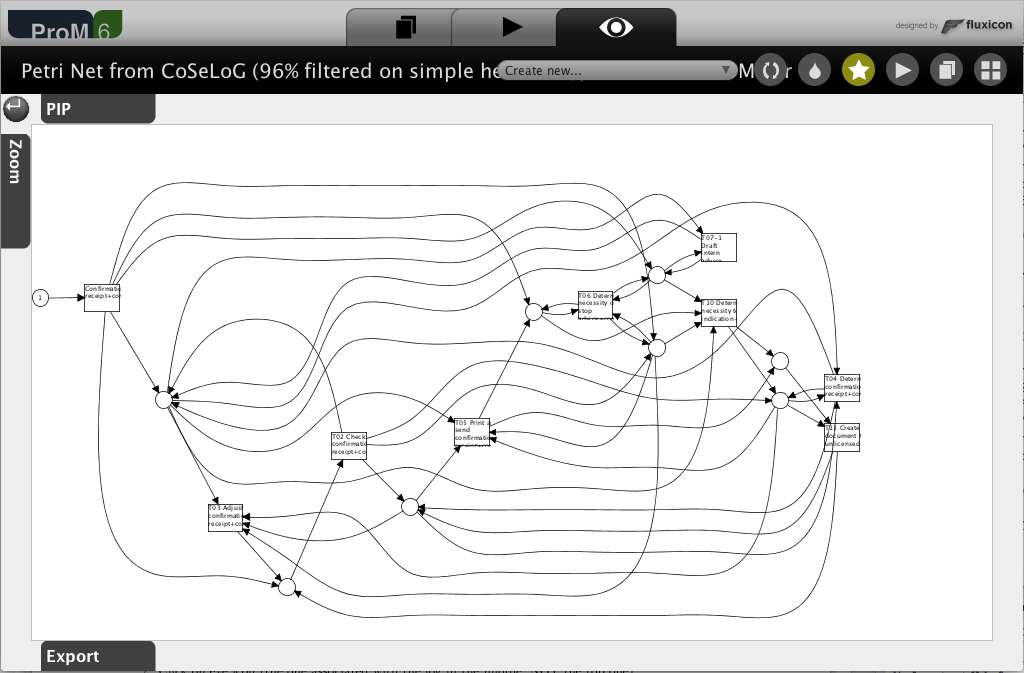
\includegraphics{CoSeLoG_Step_05_Filter96_PetriNet_ILP.png}

The main traces include:\\\textbf{1}. Start -\textgreater{} T00
-\textgreater{} T02 -\textgreater{} T05 -\textgreater{} End01 with 2
tokens remaining in ILP3 (between T00 \& T10) and ILP5 (between T00 \&
T07-1)

\textbf{2}. Start -\textgreater{} T00 -\textgreater{} T10
-\textgreater{} T11 -\textgreater{} End02 with 1 token remaining in ILP1
(between T00 \& T02)

The traces with some loops include:\\\textbf{1A}. Start -\textgreater{}
T00 -\textgreater{} T02 -\textgreater{} {[}T04{]}* -\textgreater{} T05
-\textgreater{} End01\\ After T02, there might be any number of T04
firings

\textbf{1B}. Start -\textgreater{} T00 -\textgreater{} T02
-\textgreater{} {[}T03 -\textgreater{} T02{]}* -\textgreater{} T05
-\textgreater{} End01\\ After T02, there might be any number of T03
-\textgreater{} T02 loops

\textbf{1AB}. Start -\textgreater{} T00 -\textgreater{} T02
-\textgreater{} {[}T04{]}* -\textgreater{} {[}T03 -\textgreater{}
T02{]}* -\textgreater{} T05 -\textgreater{} End01\\ After T02, there
might be any number of T04 firings and/or T03 -\textgreater{} T02 loops

\textbf{2A}. Start -\textgreater{} T00 -\textgreater{} {[}T06{]}*
-\textgreater{} T10 -\textgreater{} T11 -\textgreater{} End02

\textbf{2B}. Start -\textgreater{} T00 -\textgreater{} {[}T07-1{]}*
-\textgreater{} T10 -\textgreater{} T11 -\textgreater{} End02

\textbf{2AB}. Start -\textgreater{} T00 -\textgreater{} {[}T06{]}*
-\textgreater{} {[}T07-1{]}* -\textgreater{} T10 -\textgreater{} T11
-\textgreater{} End02

\textbf{2C1a}. Start -\textgreater{} T00 -\textgreater{} T10
-\textgreater{} T02 -\textgreater{} {[}T04{]}* -\textgreater{} {[}T03
-\textgreater{} T02{]}* -\textgreater{} T05 -\textgreater{}
End01\\\textbf{2C1b}. Start -\textgreater{} T00 -\textgreater{} T10
-\textgreater{} T11 -\textgreater{} T02 -\textgreater{} {[}T04{]}*
-\textgreater{} {[}T03 -\textgreater{} T02{]}* -\textgreater{} T05
-\textgreater{} End01

\textbf{2AC1a}. Start -\textgreater{} T00 -\textgreater{} {[}T06{]}*
-\textgreater{} T10 -\textgreater{} T02 -\textgreater{} {[}T04{]}*
-\textgreater{} {[}T03 -\textgreater{} T02{]}* -\textgreater{} T05
-\textgreater{} End01\\\textbf{2AC1b}. Start -\textgreater{} T00
-\textgreater{} {[}T06{]}* -\textgreater{} T10 -\textgreater{} T11
-\textgreater{} T02 -\textgreater{} {[}T04{]}* -\textgreater{} {[}T03
-\textgreater{} T02{]}* -\textgreater{} T05 -\textgreater{} End01

\textbf{2BC1a}. Start -\textgreater{} T00 -\textgreater{} {[}T07-1{]}*
-\textgreater{} T10 -\textgreater{} T02 -\textgreater{} {[}T04{]}*
-\textgreater{} {[}T03 -\textgreater{} T02{]}* -\textgreater{} T05
-\textgreater{} End01\\\textbf{2BC1b}. Start -\textgreater{} T00
-\textgreater{} {[}T07-1{]}* -\textgreater{} T10 -\textgreater{} T11
-\textgreater{} T02 -\textgreater{} {[}T04{]}* -\textgreater{} {[}T03
-\textgreater{} T02{]}* -\textgreater{} T05 -\textgreater{} End01

\textbf{2ABC1a}. Start -\textgreater{} T00 -\textgreater{} {[}T06{]}*
-\textgreater{} {[}T07-1{]}* -\textgreater{} T10 -\textgreater{} T02
-\textgreater{} {[}T04{]}* -\textgreater{} {[}T03 -\textgreater{}
T02{]}* -\textgreater{} T05 -\textgreater{} End01\\\textbf{2ABC1b}.
Start -\textgreater{} T00 -\textgreater{} {[}T06{]}* -\textgreater{}
{[}T07-1{]}* -\textgreater{} T10 -\textgreater{} T11 -\textgreater{} T02
-\textgreater{} {[}T04{]}* -\textgreater{} {[}T03 -\textgreater{}
T02{]}* -\textgreater{} T05 -\textgreater{} End01

All the traces that end in End01 have 2 tokens remaining as described
for Trace 1.\\All the traces that end in End02 have 1 token remaining as
described for Trace 2.

These traces should be in a table for better comprehension ?

\section{Analyze conformance with normative model in
ProM}\label{analyze-conformance-with-normative-model-in-prom}

\textbf{Approach I used}:

\begin{enumerate}
\def\labelenumi{\arabic{enumi}.}
\itemsep1pt\parskip0pt\parsep0pt
\item
  Click on ``Workspace'' icon.\\
\item
  Click on ``import\ldots{}'' button.\\
\item
  Select the normative model file.\\
\item
  Select the `PNML Petri net files' importer.\\
\item
  Click on ``Actions'' icon.\\
\item
  Search for ``Replay'' plug-in.\\
\item
  Select `Replay a Log on Petri Net for Conformance Analysis' (not the
  variant with performance!) plug-in.
\item
  Add original event log to ``Input''.\\
\item
  Click on ``Start'' button.\\
\item
  Click `yes' in the `No Final Marking' pop-up.
\item
  Select the `sink' place on the left (note: do not select `0-sink'
  etc.) and click the button `Add Place \textgreater{}\textgreater{}' to
  add the place `sink' to the candidate final marking list.
\item
  Click `Finish' in the mapping wizard.\\
\item
  Click `Finish' .\\
\item
  Click `No, I've mapped all necessary event classes' to indicate that
  some events are not present in the normative model.\\
\item
  Click `Next'.\\
\item
  Click `Finish'.
\end{enumerate}

\textbf{What I saw}:

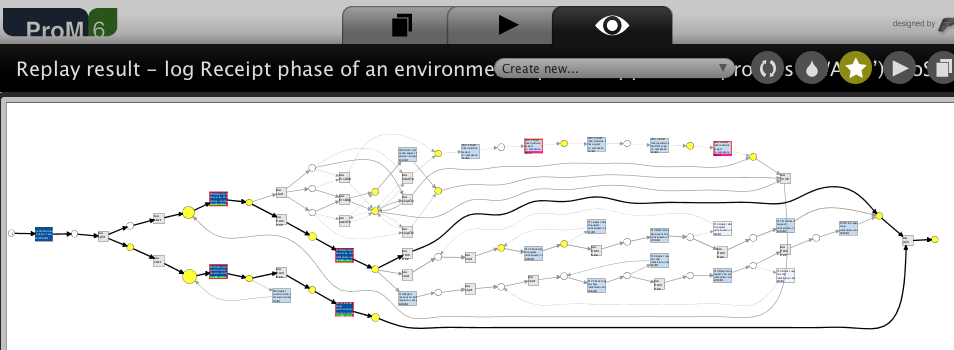
\includegraphics{CoSeLoG_Step_06_PetriNet_Normative_Conformance.png}

\emph{Transitions}: Most of the traces pass through very few ``labeled''
(tau are ``silent'') transitions: T00 -\textgreater{} T06
-\textgreater{} T10 \& T00 -\textgreater{} T04 -\textgreater{} T05. The
color darkness or ``fill'' of the transition boxes is based on the
number of traces in the event log that fire them. The numbers underneath
the label in the transition boxes refer to the number of synchronous
moves vs. ``move on model''. T13 \& T18 are never fired in this event
log.

\emph{Places}: Place size displays ``move on log'' frequency. Places
where move log occured are colored yellow. However, size of ``source''
\& ``sink'' are not adjusted. Clicking on the place displays the
underlying label. Size of places going to silent transitions are not
adjusted with frequency but are colored yellow when there are move(s) on
log.

\emph{Arcs}: The thickness of the arcs seems proportional to the
frequency of event log traces.

\textbf{My analysis}:

The replay fitness (the `trace fitness' statistic) of the event log on
the normative process model is 0.8425. T10 has the maximum deviations
(151). T06 has the minimum (125).

The transition `T06 Determine necessity of stop advice+complete' (on the
top left of the model) was tested with 1,434 traces in the event log.
Out of those 1,309 (91\%) were synchronous moves in both the model \&
log. Amongst those 1,309 traces, T06 was fired synchronously for 1,327
times (i.e.~some traces fired T06 fired multiple times). For 125 traces,
T06 was fired in the model only.

\section{Analyze resource utilization in
ProM}\label{analyze-resource-utilization-in-prom}

\textbf{Approach I used}:\\1. Click on ``Workspace'' icon.\\2. Select
event log resource.\\3. Click on ``Actions'' icon for this resource.\\4.
Search for ``Mine for a Subcontracting Social Network'' \& select
it.\\5. Keep selected default options \& click on ``Continue''
button.\\6. Click ``Start'' button.\\7. Select the following in the
Social Network view options:\\ Layout: ISOMLayout\\ Ranking:
Betweenness\\ Mouse Mode: Picking\\ Edges removed for cl\ldots{}: 3rd
tick from left\\ View options:\\ shape by degree\\ show vertex names\\
show edge\\ Group Clusters\\8. Select a resource and move it to get more
clarity in the visual.

\textbf{What I saw}:

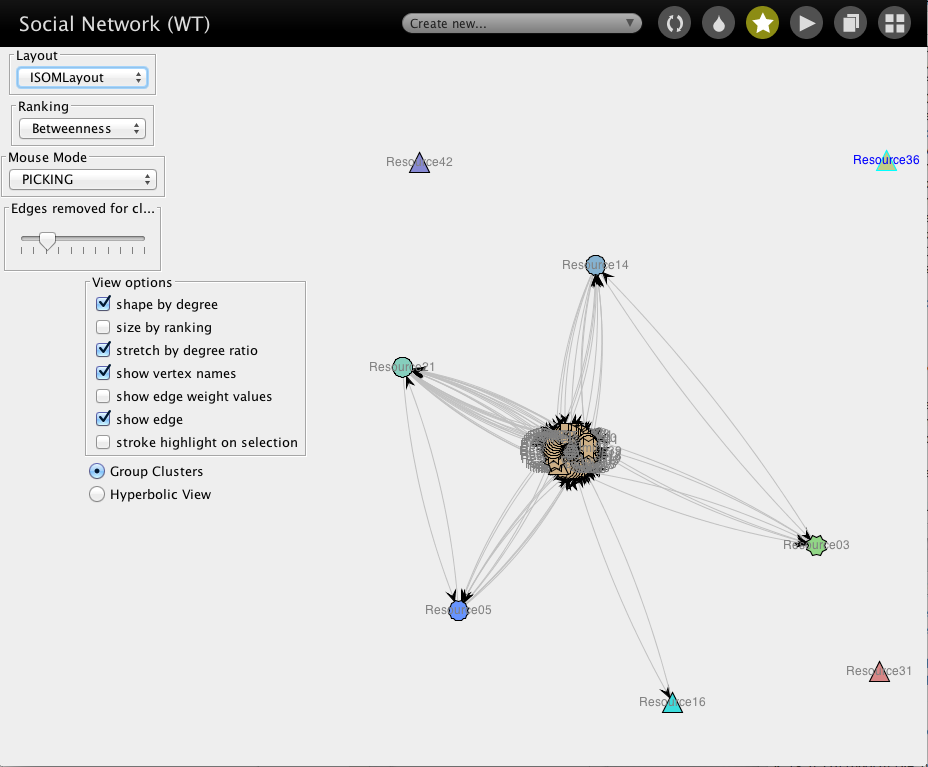
\includegraphics{CoSeLoG_Step_07_SocialNet.png}

Resources grouped by cluster, shaped by connectivity degree and edges
depicting the connectivity density.

\textbf{My analysis}:

The resources may be grouped into the following categories:\\I.
\emph{Singletons}: Resources \{31, 36 \& 42\} don't and \{16\} rarely
subcontract work.\\II. \emph{Couples}: \{05, 21\} and \{03, 14\} are
targets of subcontracting and amongst each other within the group. III.
\emph{General Pool}: All the other resources subcontract work
significantly amongst themselves.

Let's see if we can get any more granularity regarding the sub-groups in
``General Pool'' by inspecting the cases \& tasks executed by these
resources. Couldn't find an appropriate filter plug-in to do this in
ProM. Therefore, I switched to Disco and figured out that I need to
filter the event log to delete cases that the ``Singletons'' worked on
\& utilize the remaining cases to re-do this analysis.

\textbf{Approach I used}:

\begin{enumerate}
\def\labelenumi{\arabic{enumi}.}
\setcounter{enumi}{10}
\itemsep1pt\parskip0pt\parsep0pt
\item
  Click on ``Import'' icon in Disco.\\
\item
  Select the event log.\\
\item
  Click on ``Filter'' icon in the bottom left.\\
\item
  Click in the left pane to add filter.\\
\item
  Select ``Attribute - Removes events by attribute''.\\
\item
  Select ``Resource'' in the ``Filter by:'' option.\\
\item
  Select ``Mandatory'' in the ``Filtering mode:'' option.
\item
  Select ``Resource31'' only in ``Event values:'' pane.
\item
  Click on ``Apply filter'' button.
\end{enumerate}

\textbf{What I saw}:

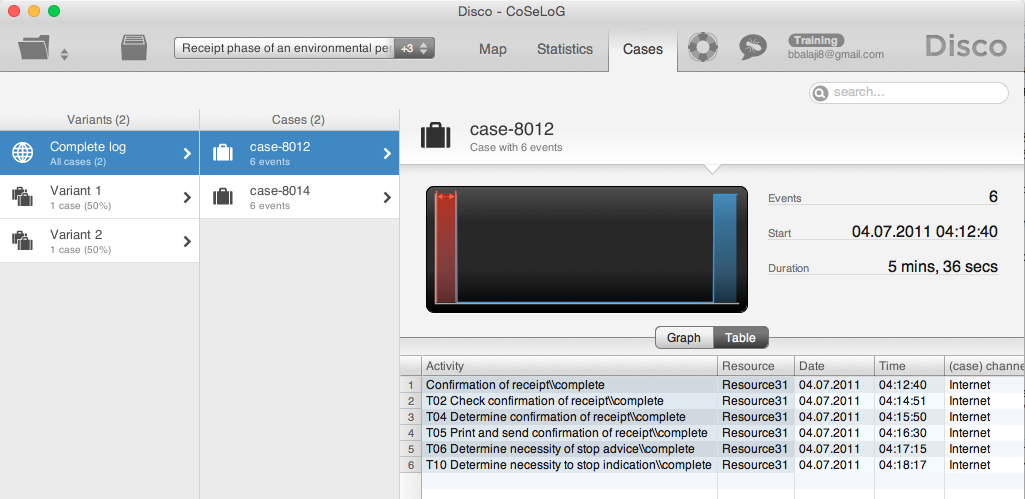
\includegraphics{CoSeLog_Step07_Filter_Resource31.png}

2 cases in which all tasks were executed by Resource31.

\textbf{My analysis}:

The ``Singletons'' worked on 4 cases (10918 for Resource 42; 4328 for
Resource 36 \& {[}8012, 8014{]} for Resource 31) only. Moreover, in each
of these cases, all the tasks were conducted by one resource. Similarly,
I also found resources \{``test'' \& ``TEST''\} who each had one case
8061 \& 8047. I excluded these cases by applying a filter \& exported
the filtered event log.

Re-did tasks 1-8 as listed above for ``Step 07: inspect resource
utilization in ProM''. The clustering in ProM suggested expanding \&
splitting the ``Singletons'' group into ``Exclusive One-timers'' and
``Occasional Helpers:'' as listed further below.

After filtering the event log to delete cases that utilize these
resources, I re-did the social networking analysis in ProM.

\textbf{What I saw}:

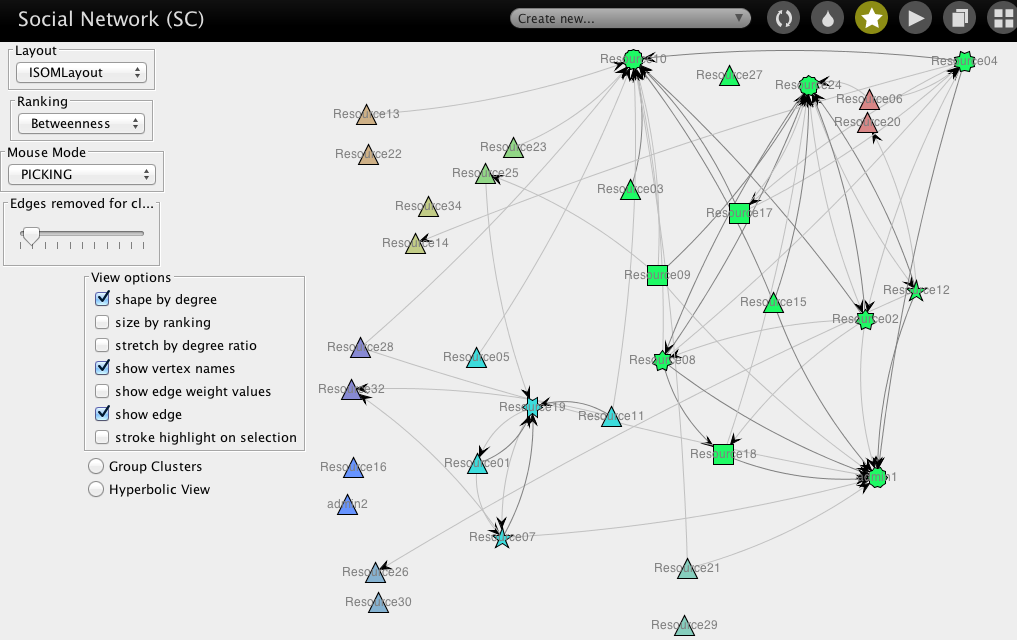
\includegraphics{CoSeLoG_Step_07_excl_one-timers_SocialNet.png}

\textbf{My analysis}:

The resources may be grouped into the following categories:\\1.
\emph{Exclusive One-timers}: Resources \{31, 36, 42, test, TEST\} have
worked on their cases exclusively (Total 6 cases).

\begin{enumerate}
\def\labelenumi{\arabic{enumi}.}
\setcounter{enumi}{1}
\item
  \emph{Occasional Helpers}: Resources \{33, 35, 37, 38, 39, 40, 41, 43,
  admin3\}\\2.1 Resources \{40, 41, 43\} have helped with one activity
  on one case each.\\2.2 Resource37 has helped with 5 activities on one
  case.\\2.3 Resource39 has helped with one activity (T02) on 2
  cases.\\2.4 Resource38 has helped with activities on 2 cases.\\2.5
  Resource admin3 has helped with one activity on 3 cases.\\2.6
  Resource33 has helped with T07-* activities on 3 cases.\\2.7
  Resource35 has helped with multiple activities on 3 cases.

  Total 17 cases.
\item
  \emph{Isolated Couples}: Resources \{{[}13, 22{]}, {[}23, 25{]},
  {[}14, 34{]}, {[}28, 32{]}, {[}16, admin2{]}, {[}26, 30{]}, {[}21,
  29{]}, {[}06, 20{]}\} occasionally are outsourced / assign work. The
  cluster sub-groups are probably based on the tasks similarity.
\item
  \emph{Workgroup A}: Resources \{01, 05, 07, 11, 19\}
\item
  \emph{Workgroup B}: Resources \{{[}10, admin1{]}, {[}04, 24{]}, {[}02,
  03, 08, 09, 12, 15, 17, 18, 27{]}\}\\5.1 Resources 10 \& admin1 are
  out-scourced work by many resources but do not assign any work to
  others.\\5.2 Resources 04 \& 24 are out-sourced work by many resources
  and occassionally assign work to others.
\end{enumerate}

For, are all users executing activities from the start of the event log,
or are some users joining later? \& are users mainly executing
particular activities or are most users executing most of the
activities?

\textbf{Approach I used}:\\21. Click on ``Workspace'' icon.\\22. Select
event log excluding cases that involve \emph{Exclusive One-timers} or
\emph{Occasional Helpers}.\\23. Click on ``Visualize'' icon for the
selected resource.\\24. Select ``XDottedChart'' by clicking on ``Create
new\ldots{}'' drop-box.\\25. Select ``Dotted Chart'' tab.\\26. Select
the following options:\\ Component: `org:resource'\\ Time: Logical\\
Case order: Occurence of first event\\27. Click on ``Apply settings''
button.

\textbf{What I saw}:

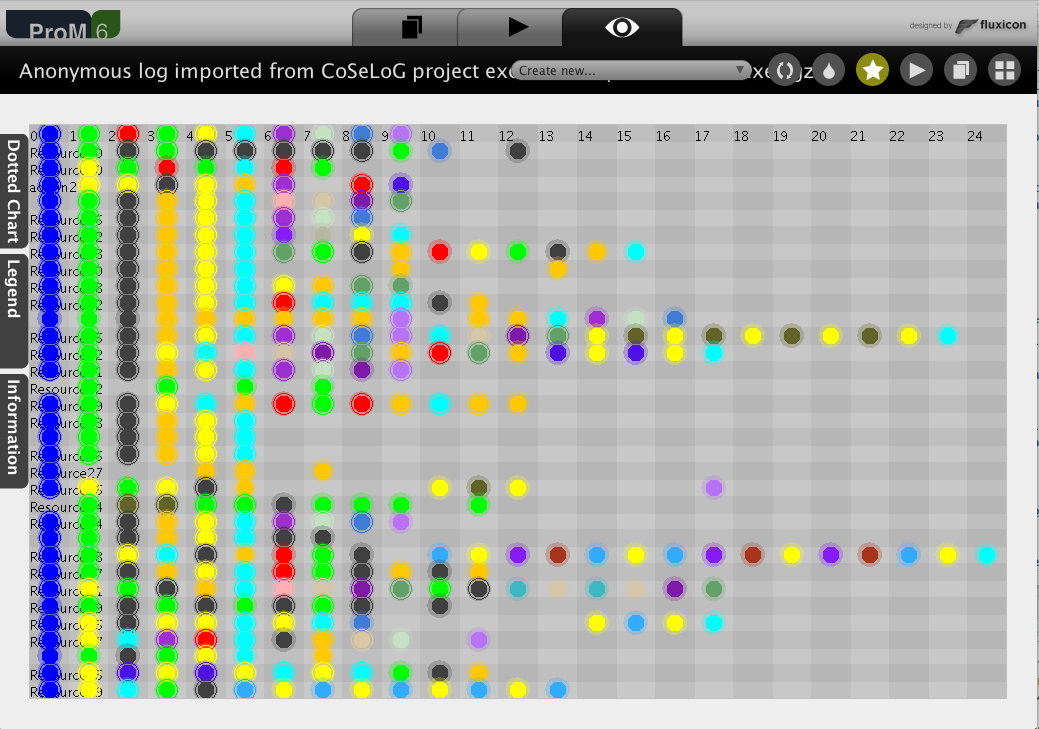
\includegraphics{CoSeLoG_Step_07_Filtered_SocialDots.png}

The resources are displayed as rows and the transitions are organized
into columns based on when the transition was executed by that resource
for a certain case. The transitions are color coded.

\textbf{My analysis}:

Most of the resources are executing activities from the start of the
event log. It's hard to identify the exceptions. I wish the chart could
be interactive (e.g.~click on a dot and obtain more information).

Most resources are executing the first few activities \{T00, T02, T06\}.
The black color is assigned to multiple activities, so it's hard to tell
whether many resources are executing these activities or only a few.
Other activities appear to be executed by only a few.

\section{Appendix}\label{appendix}

\subsection{Petri net evaluation
criteria}\label{petri-net-evaluation-criteria}

Given a Petri net and an event log, the following evaluation criteria
(not exhaustive) are useful:

\begin{enumerate}
\def\labelenumi{\arabic{enumi}.}
\item
  Fitness metrics:\\1.1 Alignment conformance of event log: ProM plug-in
  Replay a Log on Petri Net for Conformance Analysis w/ option Measuring
  fitness
\item
  Simplicity metrics:\\2.1 \# total places\\2.2 \# implicit places\\2.3
  \# silent transitions\\2.4 \# arcs\\2.5 Entropy: ProM plug-in ?\\2.6
  Minimal Description Length (MDL): ProM plug-in ?
\item
  Generalization metrics:\\3.1 Alignment conformance of ``test'' (vs.
  ``training'') event log (or cross-validation)
\item
  Precision metrics:\\4.1 Behavioral appropriateness (similar to \%
  model allowed traces present in event log ?): ProM plug-in Replay a
  Log on Petri Net for Conformance Analysis w/ option Measuring
  behavioral appropriateness
\end{enumerate}

Based on the analysis objective(s), these metrics may be assigned
appropriate weights. For this analysis, equal weights were selected
i.e.~25\% for each metric category and 20\% for the Simplicity metric
set elements (Entropy was not computed).

\subsection{Actions to run ProM plug-in ``Replay a Log on Petri Net for
Conformance
Analysis''}\label{actions-to-run-prom-plug-in-replay-a-log-on-petri-net-for-conformance-analysis}

\begin{enumerate}
\def\labelenumi{\arabic{enumi}.}
\item
  Click on ``Actions'' icon.
\item
  Search for ``Replay'' plug-in.
\item
  Select `Replay a Log on Petri Net for Conformance Analysis' (not the
  variant with performance!) plug-in.
\item
  Add event log of interest to ``Input''.
\item
  Add Petri net of interest to ``Input''.
\item
  Click on ``Start'' button.
\item
  If the selected Petri net does not have a clear ``End'' place:\\7.1.
  Click on ``Yes'' button in the dialog ``No final marking is found for
  this model. Do you want to create one?''.\\7.2. Select the appropriate
  ``End'' place(s) from the ``List of Places'' pane.\\7.3. Click on
  ``Add Place \textgreater{}\textgreater{}'' button.\\7.4. Repeat
  actions 7.2 \& 7.3 for the remaining ``End'' places. 7.5. Click on
  ``Finish'' button.
\item
  Click on ``Finish'' button in the ``Map Transitions to Event Class''
  dialog.
\item
  Click on ``No, I've mapped all necessary event classes'' in the
  ``Mapping'' dialog.
\item
  Select ``Measuring fitness'' or ``Measuring behavioral
  appropriateness''.\\10.1. For ``Measuring fitness'':\\ 10.1.1. Click
  on ``Next'' button.\\ 10.1.2. Click on ``Finish'' button.\\ 10.1.3.
  Click on ``Global Statistics (non-filtered traces)''.\\ 10.1.4.
  ``Trace Fitness'' Property displays conformance metric (referenced as
  1.1 in the ``Petri net evaluation criteria'' Appendix section).

  10.2. For ``Measuring behavioral appropriateness'':\\ 10.2.1. Click on
  ``Next'' button.\\ 10.2.2. Reduce slider for ``\# Maximum explored
  states\ldots{}'' to approx. 200 instead of 2,000 to ensure reasonable
  run-times.\\ 10.2.3. Click on ``Finish'' button.\\ 10.2.4. Click on
  ``Global Statistics (non-filtered traces)''.\\ 10.2.5. ``Behavioral
  Appropriateness'' Property displays behavioral appropriateness metric
  (referenced as 4.1 in the ``Petri net evaluation criteria'' Appendix
  section).
\end{enumerate}

Delete ?: 10. Click `yes' in the `No Final Marking' pop-up. 11. Select
the `sink' place on the left (note: do not select `0-sink' etc.) and
click the button `Add Place \textgreater{}\textgreater{}' to add the
place `sink' to the candidate final marking list. 12. Click `Finish' in
the mapping wizard.\\13. Click `Finish' .\\14. Click `No, I've mapped
all necessary event classes' to indicate that some events are not
present in the normative model.\\15. Click `Next'.\\16. Click `Finish'.

\end{document}
